% *********************************************************************
% © 2010–2026 Jeremy Sylvestre
%
% Permission is granted to copy, distribute and/or modify this document
% under the terms of the GNU Free Documentation License, Version 1.3 or
% any later version published by the Free Software Foundation; with no
% Invariant Sections, no Front-Cover Texts, and no Back-Cover Texts. A
% copy of the license is included in the appendix entitled “GNU Free
% Documentation License” that appears in the output document of this
% PreTeXt source code. All trademarks™ are the registered® marks of
% their respective owners.
%
% *********************************************************************

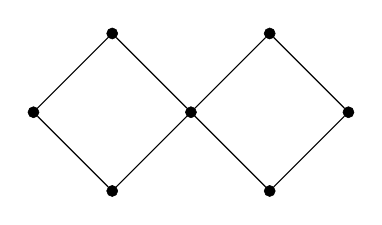
\begin{tikzpicture}[
	vertex/.style={ circle, draw, very thin, fill, inner sep=0pt, minimum size=4pt },
	vertexg/.style={ black!40!white, circle, draw, very thin, fill, inner sep=0pt, minimum size=4pt },
	vertexo/.style={ circle, draw, very thin, inner sep=0pt, minimum size=4pt }
]

\node[vertex] at (-1,1) (v3) {};
\node[vertex] at (-1,-1) (v5) {};
\node[vertex] at (1,1) (v6) {};
\node[vertex] at (1,-1) (v8) {};
\node[vertex] at (0,0) (v1) {};
\foreach \p in {v3,v5,v6,v8} \draw (v1) to (\p);
\node[vertex] at (-2,0) (v4) {};
\foreach \p in {v3,v5} \draw (v4) to (\p);
\node[vertex] at (2,0) (v7) {};
\foreach \p in {v6,v8} \draw (v7) to (\p);

\end{tikzpicture}
